\chapter{Versuch 1}
\label{chap:VERSUCH_1}

\section{Fragestellung, Messprinzip, Aufbau, Messmittel}
\label{chap:VERSUCH_1_FRAGESTELLUNG}

Bei Versuch 1 ging es um die Messung von Abständen mittels eines Entfernungssensors. 

\subsection*{Fragestellung}
	Bei der Messung soll die Standardabweichung der einzelnen Messungen ermittelt werden. Hierzu wird für 20 verschiedene Abstände jeweils eine Messung durchgeführt und die vom Sensor zurückgegebene Spannung einerseits als csv Datei gespeichert und zusätzlich handschriftlich notiert.

\pagebreak	
\subsection*{Messprinzip}
	Der Sensor sendet mit einer LED ein rotes Licht aus, das vom Objekt reflektiert und dann von einen optischen Positionssensor (OPS) wider erfasst wird. Die Leitfähigkeit des OPS ist von der Einfallposition des Lichts abhängig, so ergeben unterschiedliche Einfallspositionen unterschiedliche Spannungen, aus denen sich dann der Einfallswinkel berechnen lässt. Aus diesen kann man dann über das Triangulationsprinzip die Entfernung ermittelt.
	
	(Quellverweis einfüge: ist von der Versuchsanleitung)
	\begin{center}
	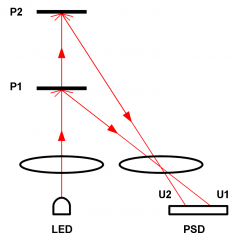
\includegraphics[scale=1]{media/triangulationGraphik.png}
	\label{Triangulation}
	\end{center}
	
	
\subsection*{Aufbau}

\begin{center}
	\includegraphics[scale=0.15]{media/aufbau.png}
	\label{Fig:Versuchsaufbau}
	\captionof{figure}{Fig: Aufbau des Versuchs}
\end{center}
	
\pagebreak	
\subsection*{Messmittel}
\ref{Versuchsaufbau}
	Zur Messung wurden folgende Messmittel benutzt:
	\begin{itemize}
		\item Sensor(Abstandmessungssensor)
		\item Osziloskop		
		\item Metermaß
		\item Brett (als Objekt dessen Abstand gemessen wird)
	\end{itemize}

\pagebreak
\section{Messwerte}
\label{chap:VERSUCH_1_MESSWERTE}
	
	
	\begin{center}
	Tabelle der von Hand notierten Werte:
	
	
	\begin{tabular}{|c|c|}
	\hline 
	Abstand in cm & Spannung in V \\ 
	\hline 
	10  & 1,363 \\ 
	\hline 
	13 & 1,212 \\ 
	\hline 
	16 & 1,078 \\ 
	\hline 
	19 & 0,973 \\ 
	
	\hline 
	22 & 0,897 \\ 
	\hline 
	25 & 0,822 \\ 
	\hline 
	28 & 0,765 \\ 
	\hline 
	31 & 0,699 \\ 
	\hline 
	34 & 0,656 \\ 
	
	\hline 
	37 & 0,637 \\ 
	\hline 
	40 & 0,599 \\ 
	\hline 
	43 & 0,560 \\ 
	\hline 
	46 & 0,541 \\ 
	
	\hline 
	49 & 0,523 \\ 
	\hline 
	52 & 0,523 \\ 
	\hline 
	55 & 0,504 \\ 
	\hline 
	58 & 0,485 \\ 
	
	\hline 
	61 & 0,485 \\ 
	\hline 
	64 & 0,485 \\ 
	\hline 
	67 & 0,485 \\ 
	\hline 
	70 & 0,466 \\ 
	\hline 
	\end{tabular} 
	\end{center}
\captionof{table}{Tab: gemessene Werte}
\label{Tabelle: gemessene Werte}
	
\pagebreak
\section{Auswertung}
\label{chap:VERSUCH_1_AUSWERTUNG}


\subsection{Prinzip der Auswertung}
\label{Prinzip der Auswertung}
Ziel ist es, die Standardabweichung der Messung zu ermitteln und 
	Zunächst werden aus der CSV Dateien die Mittelwerte für die gemessenen Spannungswerte ermittelt, der als Näherung an den wahren  Wert verwendet wird.
Formel für den Mittelwert:
	\begin{equation}
		\bar{x} = \frac{1}{n}\sum_{i=1}^nx_i
	\end{equation}
	
	Erläuterung:
	\begin{itemize}
	\item $\bar{x}$ ist der arithmetische Mittelwert
	\end{itemize}
	
Aus diesen Mittelwert lässt sich dann die Standardabweichung nach folgender Formel ermittelt:
\\
\begin{equation}
		s_{\bar{x}} = \sqrt{\frac{1}{n(n-1)}\sum_{i=1}^n(\bar{x}-x_i)^2} =\frac{s}{\sqrt{n}}
\end{equation}
\\

\begin{itemize}
\item $s_{\bar{x}}$ ist die Standardabweichung für den Mittelwert
\item s ist die empirische Standardabweichung
\item $\bar{x}$ ist der Mittelwert
\end{itemize}

	
\pagebreak
\subsection{Tabelle: Mittelwerte und Standardabweichung}
\label{chap: Tabllen_Auswertung}
\begin{center}

\begin{tabular}{|c|c|c|c|}
\hline 
Entfernung in cm & Spannung in V & Mittelwert der Spannung in V & Standardabweichung  \\ 
\hline 
10 & 1,363 & 1.341 & 0.028 \\ 
\hline 
13 & 1,212 & 1.196 & 0.017 \\ 
\hline 
16 & 1,078 & 1.078 & 0.017 \\ 
\hline 
19 & 0,973 & 0.983 & 0.017 \\ 

\hline 
22 & 0,897 & 0.907 & 0.017 \\ 
\hline 
25 & 0,822 & 0.807 & 0.017 \\ 
\hline 
28 & 0,765 & 0.749 & 0.018 \\ 
\hline 
31 & 0,699 & 0.709 & 0.018 \\ 
\hline 
34 & 0,656 & 0.671 & 0.017 \\ 
\hline 

37 & 0,637 & 0.632 & 0.018 \\ 
\hline 
40 & 0,599 & 0.612 & 0.017 \\ 
\hline 
43 & 0,560 & 0.575 & 0.017 \\ 
\hline 
46 & 0,541 & 0.535 & 0.017 \\ 

\hline 
49 & 0,523 & 0.496 & 0.017 \\ 
\hline 
52 & 0,523 & 0.473 & 0.017 \\ 
\hline 
55 & 0,504 & 0.453 & 0.017 \\ 
\hline 
58 & 0,485 & 0.434 & 0.018 \\ 

\hline 
61 & 0,485 & 0.396 & 0.018 \\ 
\hline 
64 & 0,485 & 0.375 & 0.018 \\ 
\hline 
67 & 0,485 & 0.356 & 0.018 \\ 
\hline 
\end{tabular} 
\label{Tabelle: Mittelwerte und Standardabweichung}
\captionof{table}{Tab: gefundene Mittelwerte und Standardabweichung}
\end{center}

\pagebreak
\subsection{Plots}
\label{Graphik: Plots vom Mittelwert und Standardabweichung}

	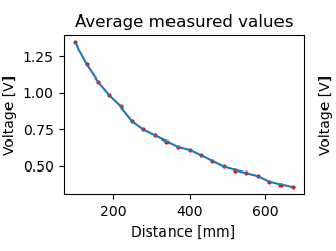
\includegraphics[scale=1]{media/avrg.png}
	\captionof{figure}{Fig: Plot zum Mittelwert}

	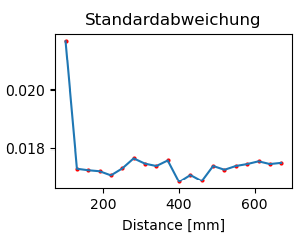
\includegraphics[scale=1]{media/stdabw.png}
	\captionof{figure}{Fig: Plot zum Standardabweichung}

	
\section{Interpretation}

Die Standardabweichung ist bei einer Entfernung von 10 cm am höchsten, fast doppelt so hoch wie bei den anderen Messungen, daraus lässt sich schließen das er der ungenauste Wert ist.
Bei den andern Werten bleibt die Standardabweichung sehr konstant.
Die Standardabweichung sollte idealerweise nur vom Rauschen, also zufälligen Störungen durch die Umgebung, verursacht werden. Da die Standardabweichung bei einen Wert deutlich höher ist als bei den anderen vermute ich das es bei dieser zu einer stärkeren Störung von außen kam, z.B. durch anstoßen des Sensors oder Lichteinfall.
	
\label{chap:VERSUCH_1_INTERPRETATION}
